% System Overview Diagram for GameWeb
% An LLM-driven 2D game generation platform
% Compile with: pdflatex system_overview.tex
\documentclass[border=8pt]{standalone}
\usepackage{tikz}
\usepackage{amsmath,amssymb}
\usetikzlibrary{arrows.meta, positioning, fit, backgrounds, calc, shapes.geometric}

\begin{document}
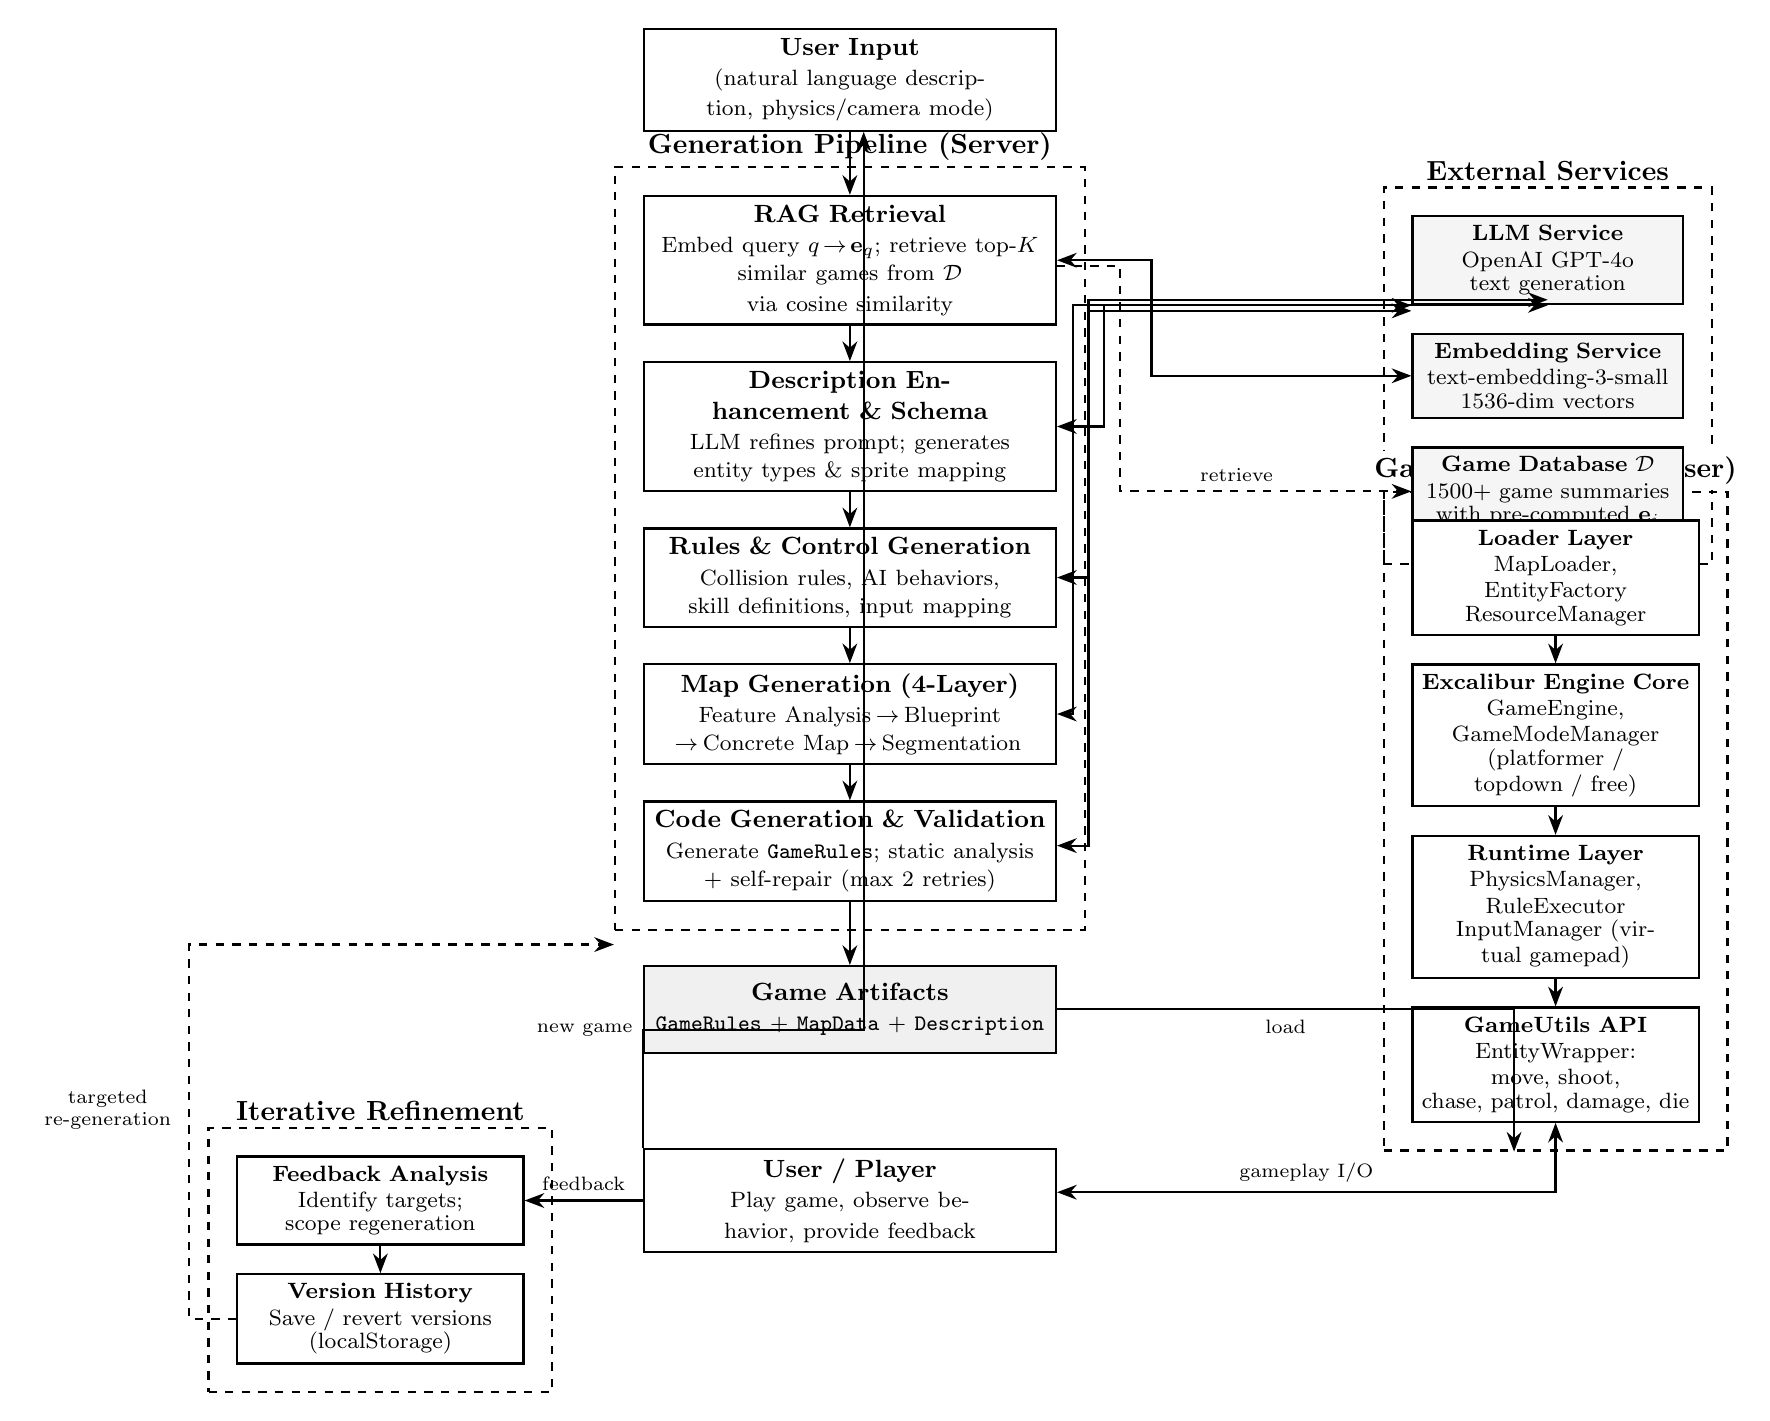
\begin{tikzpicture}[
    % === Node styles ===
    mainblock/.style={
        rectangle, draw=black, thick,
        text width=5cm, minimum height=1.1cm,
        align=center, font=\small,
        fill=white
    },
    subblock/.style={
        rectangle, draw=black, thick,
        text width=3.4cm, minimum height=0.85cm,
        align=center, font=\footnotesize,
        fill=white
    },
    extblock/.style={
        rectangle, draw=black, thick,
        text width=3.2cm, minimum height=0.85cm,
        align=center, font=\footnotesize,
        fill=gray!8
    },
    groupbox/.style={
        rectangle, draw=black, dashed, thick,
        inner sep=10pt
    },
    % === Arrow styles ===
    arr/.style={-{Stealth[length=2.5mm]}, thick},
    darr/.style={{Stealth[length=2.5mm]}-{Stealth[length=2.5mm]}, thick},
    dasharr/.style={-{Stealth[length=2.5mm]}, thick, dashed},
    % === Label style ===
    glabel/.style={font=\small\bfseries, fill=white, inner sep=2pt},
]

% ==============================================
% TOP: User Input
% ==============================================
\node[mainblock] (input) at (0, 0) {
    \textbf{User Input}\\
    {\footnotesize (natural language description, physics/camera mode)}
};

% ==============================================
% LEFT COLUMN: Generation Pipeline
% ==============================================
\node[mainblock, below=0.8cm of input] (rag) {
    \textbf{RAG Retrieval}\\
    {\footnotesize Embed query $q \!\rightarrow\! \mathbf{e}_q$; retrieve top-$K$}\\[-1pt]
    {\footnotesize similar games from $\mathcal{D}$ via cosine similarity}
};

\node[mainblock, below=0.45cm of rag] (enhance) {
    \textbf{Description Enhancement \& Schema}\\
    {\footnotesize LLM refines prompt; generates}\\[-1pt]
    {\footnotesize entity types \& sprite mapping}
};

\node[mainblock, below=0.45cm of enhance] (rules) {
    \textbf{Rules \& Control Generation}\\
    {\footnotesize Collision rules, AI behaviors,}\\[-1pt]
    {\footnotesize skill definitions, input mapping}
};

\node[mainblock, below=0.45cm of rules] (mapgen) {
    \textbf{Map Generation (4-Layer)}\\
    {\footnotesize Feature Analysis $\!\rightarrow\!$ Blueprint}\\[-1pt]
    {\footnotesize $\!\rightarrow\!$ Concrete Map $\!\rightarrow\!$ Segmentation}
};

\node[mainblock, below=0.45cm of mapgen] (codegen) {
    \textbf{Code Generation \& Validation}\\
    {\footnotesize Generate \texttt{GameRules}; static analysis}\\[-1pt]
    {\footnotesize + self-repair (max 2 retries)}
};

% Pipeline group box
\begin{scope}[on background layer]
\node[groupbox, fit=(rag)(enhance)(rules)(mapgen)(codegen),
    label={[glabel, anchor=south]above:{\normalsize Generation Pipeline (Server)}}
] (pipebox) {};
\end{scope}

% Pipeline arrows
\draw[arr] (input) -- (rag);
\draw[arr] (rag) -- (enhance);
\draw[arr] (enhance) -- (rules);
\draw[arr] (rules) -- (mapgen);
\draw[arr] (mapgen) -- (codegen);

% ==============================================
% RIGHT-TOP: External Services
% ==============================================
\node[extblock, right=4.5cm of rag] (llm) {
    \textbf{LLM Service}\\
    {\footnotesize OpenAI GPT-4o}\\[-1pt]
    {\footnotesize text generation}
};

\node[extblock, below=0.35cm of llm] (embed) {
    \textbf{Embedding Service}\\
    {\footnotesize text-embedding-3-small}\\[-1pt]
    {\footnotesize 1536-dim vectors}
};

\node[extblock, below=0.35cm of embed] (gamedb) {
    \textbf{Game Database $\mathcal{D}$}\\
    {\footnotesize 1500+ game summaries}\\[-1pt]
    {\footnotesize with pre-computed $\mathbf{e}_i$}
};

\begin{scope}[on background layer]
\node[groupbox, fit=(llm)(embed)(gamedb),
    label={[glabel, anchor=south]above:{\normalsize External Services}}
] (extbox) {};
\end{scope}

% Pipeline <-> External arrows
\draw[darr] (rag.east) -- ++(1.2, 0) |- (embed.west)
    node[pos=0.15, above, font=\scriptsize] {};
\draw[dasharr] ([yshift=-2pt]rag.east) -- ++(0.8, 0) |- (gamedb.west)
    node[pos=0.7, above, font=\scriptsize] {retrieve};
\draw[darr] (enhance.east) -- ++(0.6, 0) |- (llm.south west);
\draw[darr] (rules.east) -- ++(0.4, 0) |- ([yshift=-2pt]llm.south west);
\draw[darr] (mapgen.east) -- ++(0.2, 0) |- (llm.south);
\draw[darr] ([yshift=2pt]codegen.east) -- ++(0.4, 0) |- ([yshift=2pt]llm.south);

% ==============================================
% CENTER: Game Artifacts
% ==============================================
\node[mainblock, below=0.8cm of codegen, fill=gray!12] (artifacts) {
    \textbf{Game Artifacts}\\
    {\footnotesize \texttt{GameRules} + \texttt{MapData} + \texttt{Description}}
};

\draw[arr] (codegen) -- (artifacts);

% ==============================================
% RIGHT-BOTTOM: Game Runtime Engine
% ==============================================
\node[subblock, right=4.5cm of rules] (loader) {
    \textbf{Loader Layer}\\
    {\footnotesize MapLoader, EntityFactory}\\[-1pt]
    {\footnotesize ResourceManager}
};

\node[subblock, below=0.35cm of loader] (engine) {
    \textbf{Excalibur Engine Core}\\
    {\footnotesize GameEngine, GameModeManager}\\[-1pt]
    {\footnotesize (platformer / topdown / free)}
};

\node[subblock, below=0.35cm of engine] (runtime) {
    \textbf{Runtime Layer}\\
    {\footnotesize PhysicsManager, RuleExecutor}\\[-1pt]
    {\footnotesize InputManager (virtual gamepad)}
};

\node[subblock, below=0.35cm of runtime] (api) {
    \textbf{GameUtils API}\\
    {\footnotesize EntityWrapper: move, shoot,}\\[-1pt]
    {\footnotesize chase, patrol, damage, die}
};

\begin{scope}[on background layer]
\node[groupbox, fit=(loader)(engine)(runtime)(api),
    label={[glabel, anchor=south]above:{\normalsize Game Runtime (Browser)}}
] (rtbox) {};
\end{scope}

% Internal engine arrows
\draw[arr] (loader) -- (engine);
\draw[arr] (engine) -- (runtime);
\draw[arr] (runtime) -- (api);

% Artifacts -> Engine
\draw[arr] (artifacts.east) -| ([xshift=-15pt]rtbox.south)
    node[pos=0.25, below, font=\scriptsize] {load};

% ==============================================
% BOTTOM: User & Feedback Loop
% ==============================================
\node[mainblock, below=1.2cm of artifacts] (user) {
    \textbf{User / Player}\\
    {\footnotesize Play game, observe behavior, provide feedback}
};

% User <-> Engine
\draw[darr] (api.south) |- ([yshift=3pt]user.east)
    node[pos=0.75, above, font=\scriptsize] {gameplay I/O};

% Feedback
\node[subblock, left=1.5cm of user] (feedback) {
    \textbf{Feedback Analysis}\\
    {\footnotesize Identify targets;}\\[-1pt]
    {\footnotesize scope regeneration}
};

\node[subblock, below=0.35cm of feedback] (version) {
    \textbf{Version History}\\
    {\footnotesize Save / revert versions}\\[-1pt]
    {\footnotesize (localStorage)}
};

\begin{scope}[on background layer]
\node[groupbox, fit=(feedback)(version),
    label={[glabel, anchor=south]above:{\normalsize Iterative Refinement}}
] (itbox) {};
\end{scope}

\draw[arr] (user) -- (feedback)
    node[midway, above, font=\scriptsize] {feedback};
\draw[arr] (feedback) -- (version);

% Feedback loop arrow back to pipeline
\draw[dasharr] (version.west) -- ++(-0.6, 0) |- ([yshift=-5pt]pipebox.south west)
    node[pos=0.28, left, font=\scriptsize, text width=1.8cm, align=center] {targeted\\re-generation};

% User Input from user
\draw[arr] (user.north west) -- ++(0, 1.5) -| ([xshift=5pt]input.south)
    node[pos=0.0, left, font=\scriptsize] {new game};

\end{tikzpicture}
\end{document}
